\documentclass[12pt,a4pape, fullpage]{article}
\usepackage[
margin=1.5cm,
includefoot,
footskip=30pt,
]{geometry}
\usepackage[utf8]{inputenc}
%\usepackage[T1]{fontenc}
\usepackage{amsmath}
\usepackage{amsfonts}
\usepackage{amssymb}
\usepackage{graphicx}
\usepackage{comment}
\usepackage{natbib}
\usepackage{lineno}
\usepackage{url}

\bibliographystyle{evolution.bst}

\newcommand{\norm}[1]{\left\lVert#1\right\rVert}
\newcommand{\normsq}[1]{\left\lVert#1\right\rVert^2}


\newcommand{\MX}{\mathbf{X}} %uncentered data
\newcommand{\MC}{\mathbf{C}} %centering
\newcommand{\MY}{\mathbf{Y}} %centered data
\newcommand{\MF}{\mathbf{F}_2} %F2-distance matrix
\newcommand{\MFT}{\mathbf{F}_3} %F3-distance matrix
\newcommand{\MP}{\mathbf{P}} % PCs
\newcommand{\ML}{\mathbf{L}} % loadings
\newcommand{\MK}{\mathbf{K}} % Kernel
\newcommand{\MSINGULAR}{\mathbf{\Sigma}} % Singular values matrix
\newcommand{\MEIGEN}{\mathbf{\Lambda}} % Eigenvalue matrix


\newcommand{\MEAN}{\boldsymbol{\mu}} % Kernel
\begin{document}
\section{Introduction}
About 15\% of genetic variation in humans can be explained by population structure \cite{lewontin1972, barbujani1997, rosenberg2003}, but the information contained in these 15\% is sufficient to study the genetic diversity and history in great detail \cite{edwards2003}. For some data sets it is possible to predict an individuals origin at a resolution of a few hundred kilometers \cite{novembre2008, leslie2015}, and direct-to-consumer-genetics companies are using this variation to analyze the genetic data of millions of customers.

In Lewontin's pioneering analysis, he found that less than half (6\%), of that variation could be attributed to the continental-scale groups he called races, it seemed  which he used to claim that ''racial classification is (...) seen to be of virtually no genetic or taxonomic significance``.

One related question is how discrete human populations are. While human genetic differentiation generally increases with geographic distance \cite{ramachandran2005, rosenberg2007}, this increase is not uniform. Obstacles to migration,  such as oceans, mountains or deserts do frequently cause discontinuities in population structure \cite{peter2020a}. Thus, while barriers to gene flow rarely are absolute, segregation policies by (perceived) ethnic or racial ancestry frequently cause local small-scale population differentiation that persist to the present day.

Thus, it frequently a useful analysis tool to think of populations as discrete units. For example, even though the underlying population structure may be continuous, sampling is not; and when quantifying ascertainment and sampling biases, or when discussing population structure it is often helpful to pretend populations are discrete, even though the underlying structure is typically more complex. This leads to challenges both in data interpretation and communication, and often researchers will analyze a data set both using methods that assume population structure is discrete, and methods where this assumption does not need to be made.

One discrete framework for the analysis of human population structure that gained a lot of traction in the last decade are the $F$-statistics \textit{sensu} Patterson \cite{patterson2012, peter2016}. This framework treats populations as discrete units in the analysis, and allows for a variety of tests for treeness. Using this framwork, the vast majority of present-day human populations are admixed \cite{pickrell2014}. Yet, this framework starts with the assumption that admixture is i) rare and ii) discrete.

However, $F$-statistics are not restricted to discrete populations. Indeed, as they can be written as functions of allele frequency variances, or expected pairwise coalescence times, statistics that can be calculated under a wide range of demographic models \cite{peter2016}. Indeed, as they reflect inner products, they can be generalized to Euclidean space \cite{oteo2021} (or any Hilbert space, although we won't pursue that here).
Here, I explore these links between $F$-statistics and Euclidean spaces to establish connections between $F$-statistics and PCA. This allows direct interpretation of admixture in scenarios where population structure might not be discrete.




Particularly for the analysis of ancient DNA, two approaches have been proven to be particularly useful: one are global summary analyses, such as Structure \citep{pritchard2000, alexander2009} Principal Component Analysis (PCA) \citep{cavalli-sforza1994, reich2008, novembre2008, mcvean2009} and classical multidimensional scaling (MDS) \cite{fu2016, malaspinas_bammds}. Typically, these methods assume that population structure is \emph{sparse}, so that a low-rank approximation with few underlying ``components'' is sufficient to model population structure See e.g. \cite{engelhardt2010} for a useful perspective how these approaches are related.

Facing a novel data set, PCA or MDS are often the first analyses (beyond quality controls) a researcher performs, in order to obtain insights in the general population structure they are faced with. In order to answer more specific questions and to test specific hypotheses, the $F$-statistic framework of \cite{patterson2012} has been proven particularly powerful (see also \cite{peter2016} for a more gentle introduction). In the $F$-statistic framework, usually only a small number of populations are used at once, to e.g. test for treeness and find closely related populations.

Even though these two approaches are considered in almost every ancient DNA paper, links between the inferences made from them are usually only compared qualitatively. In this paper, our goal is to show that PCA and $F$-statistics are in fact closely related by construction, and use a very similar summary of the data. 





	
\section{Theory}
In this section, I will give a very brief introduction to $F$-statistics and PCA. A more detailed technical introduction of PCA is given in XXXXX, and a useful guide to interpretation is \cite{cavalli-sforza1994}.

\subsection{Introduction to PCA}
Let us assume we have some genotype data summarized in a matrix $\MX$ whose entry $x_{ij}$ reflects the allele frequency of the $i$-th population at the $j$-th genotype. If we have $S$ SNPs and $n$ populations, $\MX$ will have dimension $n \times S$. As a population may be represented by just one (pseudo-)haploid or diploid individual, there is no conceptual difference between these cases and I will
refer to populations as unit for analysis, for simplicity. Since the allele
frequencies are between zero and one, we can interpret each Population $X_i$
of $\MX$ as a point in $[0, 1]^S$, the \emph{data space} of all possible allele frequencies on our markers.
	
The goal of PCA is to find a low-dimensional subspace $\mathbb{R}^K$ of the data that explains most of the variation in the data. $K$ is at most $n-1$, but the historical processes that generated often result in \emph{sparse} data \citep{engelhardt2010,
patterson2012}, so that $K \ll n$; for visualization $K=2$ is frequently used (see Fig. \ref{fig:pca_explanation} for an intuitive explanation). 
	
	\begin{figure}
		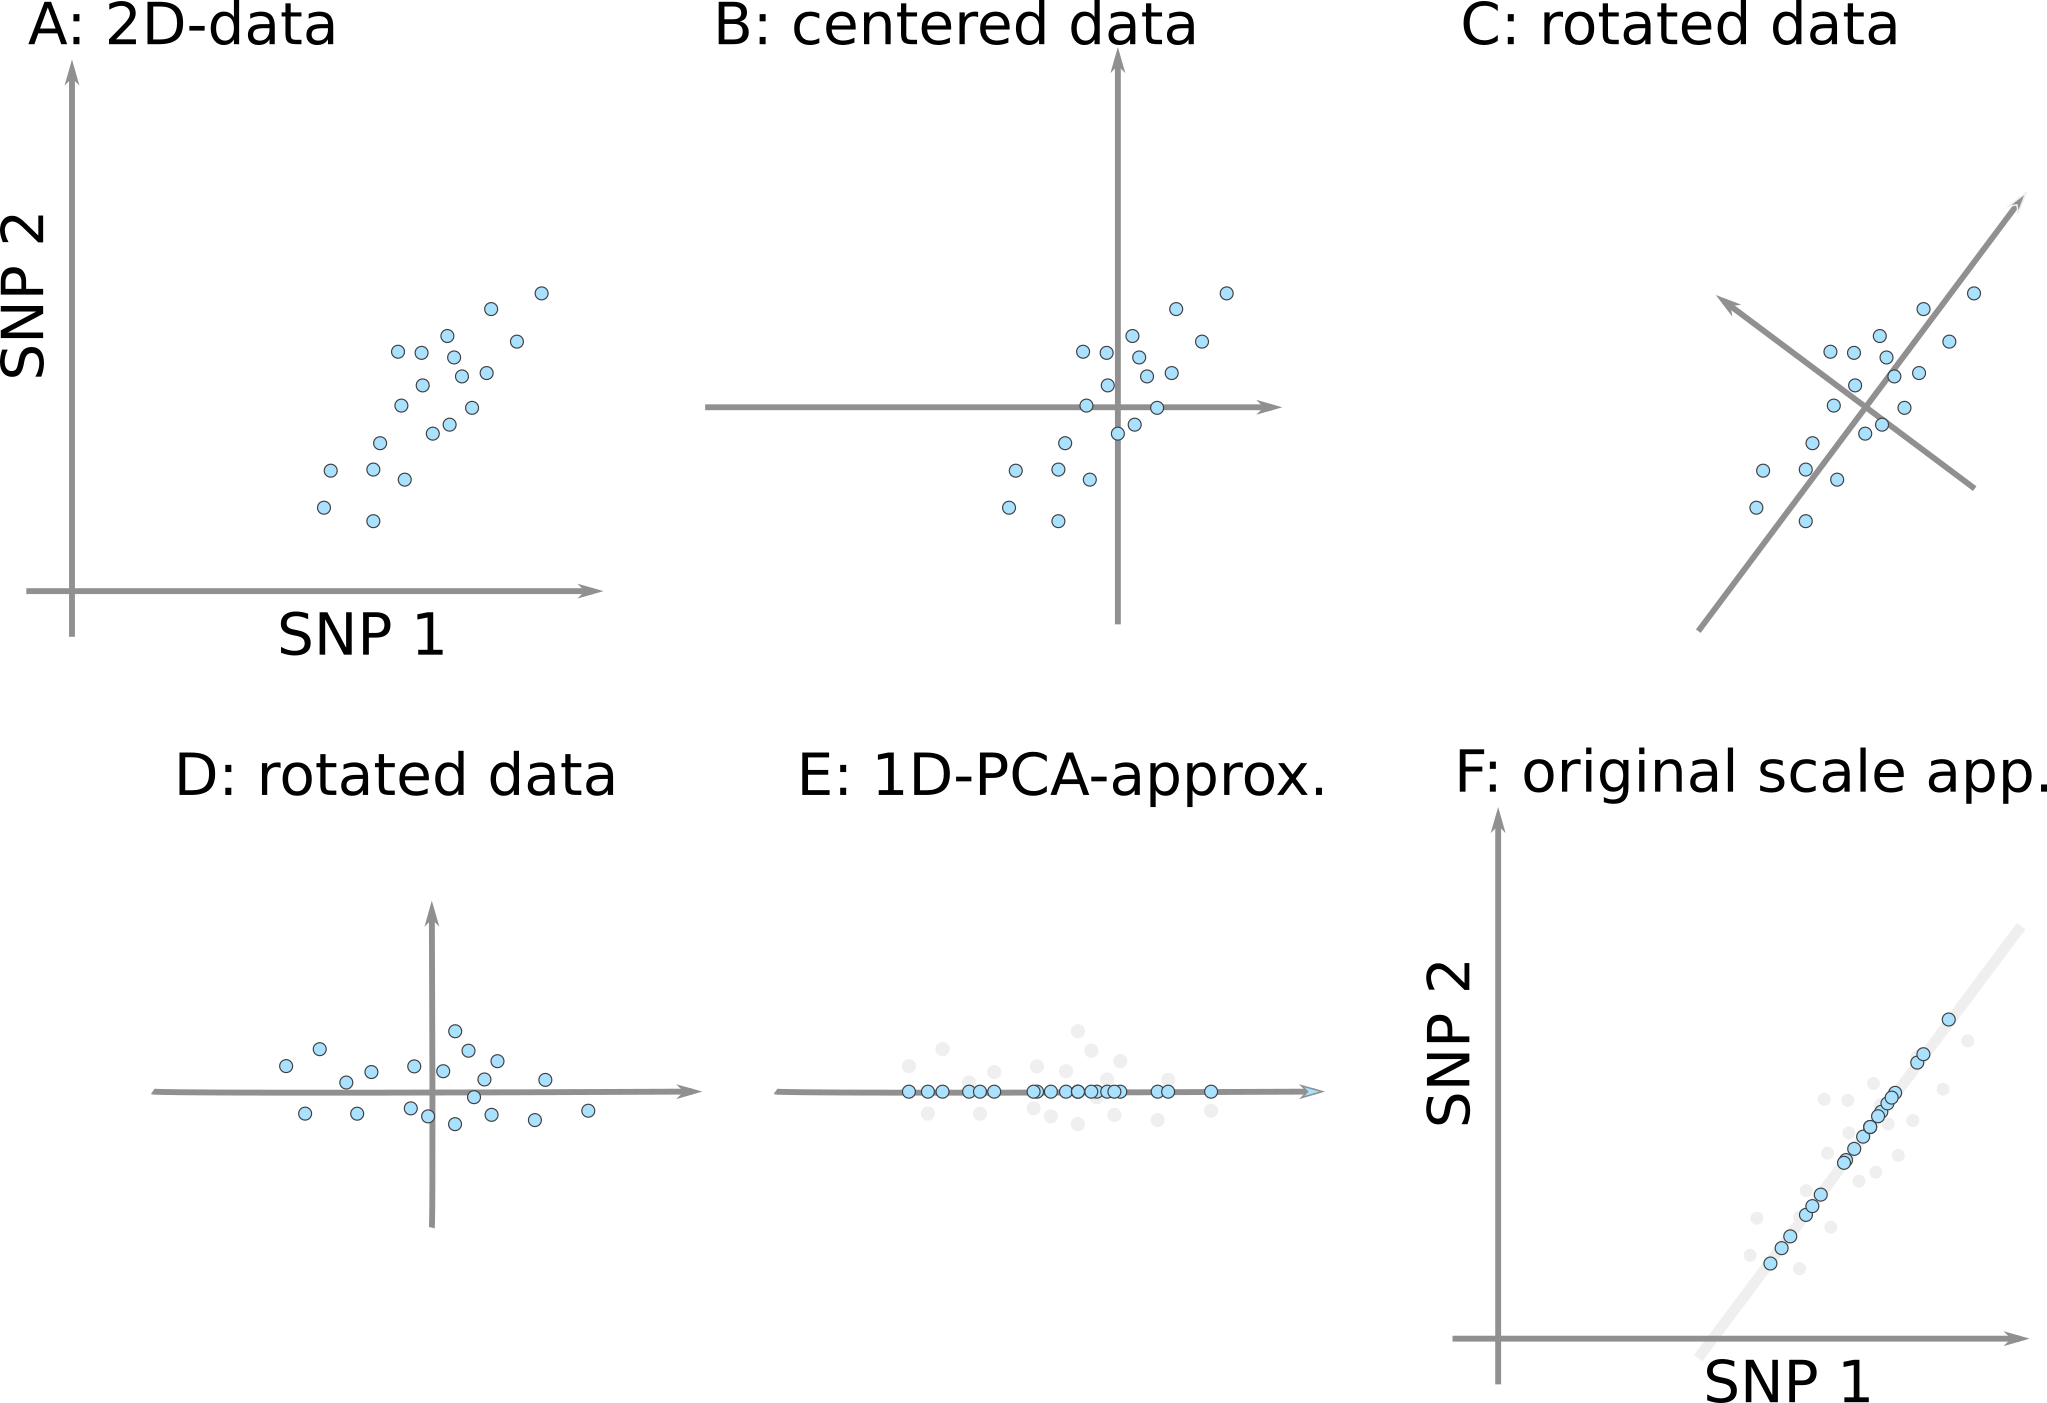
\includegraphics[width=\textwidth]{pca_explanation.png}
		\caption{Basic Idea of PCA from 2D to 1D representation. A: Allele frequencies from different populations (blue dots) at two SNPs. A PCA is performed by centering the data (B), and rotating it (B) such that the first PC explains the majority of variation in the data, and the second PC is orthognal to the first, and explains the residual. A lower-dimensional approximation (in this case 1D) can be achieved by just keeping the first PC (E); which can be translated back to the original data space by inverting the rotation and centering (F).}
		\label{fig:pca_explanation}
	\end{figure}
	
There are several algorithms that are used to calculate a PCA in practice,
   the most common one is based on singular value decomposition. In this approach, we first mean-center $\MX$, obtaining a centered matrix $\MY$
	\begin{equation*}
	y_{il} = x_{il} - \mu_l
	\end{equation*}
	where $\mu_l$ is the mean allele frequency at the $l$-th locus.
	
	PCA can then be written as
	
	\begin{equation}
	\MY = \MC\MX = \mathbf{U} \MSINGULAR \mathbf{V}^T = \MP\ML\text{,}
	\end{equation}
	
	where $\MC = \mathbf{I} -\frac{1}{n}\mathbf{1}$ is a centering matrix that subtracts row means, with $\mathbf{I}, \mathbf{1}$  the identity matrix and a matrix of ones, respectively. The orthogonal matrix of principal components $\MP=\mathbf{U}\MSINGULAR$ has size $n \times n$ and is used to reveal population structure. The loadings $\ML=\mathbf{V}^T$ are an orthonormal matrix of size $n \times k$, its rows give the contribution of each SNP to each PC, it is often useful to look for outliers that might be indicative of selection \cite[e.g][]{francois2010}.
	
	In many  implementations \citep[e.g]{patterson2006}, SNPs are weighted by
    the inverse of their standard deviation. As this weighting often makes little
    difference in practice \citep{mcvean2009}, I will assume throughout that SNPs
    are unweighted.

\subsection{Introduction to $F$-statistics}
PCA is typically used to model population structure between many populations. $F$-statistics take the opposite approach, revealing the relationship between just two,  three or four populations at a time. 

\begin{subequations}
	\begin{align}
	F_2(X_1, X_2) &=& \sum_{l=1}^S(x_{1l - x{2l}})^2 &=& \normsq{X_1, X_2}\\
	F_3(X_1; X_2, X_3) &=& \sum_{l=1}^S(x_{1l} - x_{2l})(x_{1l} - x_{3l}) &=& \langle X_1 - X_2, X_1 - X_3 \rangle\\	
	F_4(X_1, X_2; X_3, X_4) &=& \sum_{l=1}^S(x_{1l} - x_{2l})(x_{3l} - x_{4l}) &=& \langle X_1 - X_2, X_3 - X_4 \rangle	\text{,}
	\end{align}
\end{subequations}
where $\norm{\cdot}$ denotes the Euclidean norm and $\langle \cdot, \cdot \rangle$ denotes the dot product.

$F$-statistics have been primarily motivated in the context of trees and admixture graphs \citep{patterson2012}, although they can be calculated under most population genetic models \citep{peter2016}. Most commonly, $F_3$ and $F_4$ are interpreted as admixture tests: Negative values of  $F_3(X_1; X_2, X_3) < 0$ are interpreted that $X_1$ is a mixture between populations (related to) $X_2$ and $X_3$. Similarly if populations are related as a tree, then $F_4(X_1, X_2; X_3, X_4) =0$. Alternatively, $F_2$, $F_3$ and $F_4$ are all used to measure genetic similarity. $F_2(X_1, X_2)$ represents the variance in allele frequency between populations $X_1$ and $X_2$, which is a measure of genetic drift. The outgroup-$F_3$-statistic $F_3(X_O; X_U, X_i)$ is used if we have an unknown population $X_U$, and want to find its closest relatives from a panel of populations $X_i$. The highest values of $F_3$ indicate the population $X_i$ most closely related to $X_U$. Including an outgroup $X_0$ allows correction for sampling-time difference, which are common in applications on ancient DNA. Finally, $F_4(X_1, X_2; X_3, X_4)$ is used to measure the length of the internal branch on the tree connecting these four populations. It is used to reconstruct admixture graphs \cite{patterson2012, lipson2013} and to estimate admixture proportions \citep{petr2019, harney2020}.

Here, we are interested in interpreting the $F$-statistics in the data space $\mathbb{R}^S$, and compare it with PCA. For a thorough introduction of interpreting $F$-statistics in data space, see \cite{oteo-garcia2021}.
	
\paragraph{Principal components from $F$-statistics}
The principal components can be directly calculated from $F$-statistics using multidimensional scaling. Suppose we calculate the pairwise $F_2(X_i, X_j)$ between all $n$ populations, and collect them in a matrix $\MF$. We can obtain the principal components from this matrix by double-centering it, so that its row and column means are zero, and perform an eigendecomposition of the resulting matrix:
\begin{equation}
\MP\MP^T = - \frac{1}{2}\MC\MF\MC \text{.} \label{eq:mds}
\end{equation}

\section{$F$-statistics in PCA-space}
As shown by e.g. \cite{oteo-garcia2021}, $F$-statistics can be thought of as inner products in Euclidean space, and $F_2$ is an (estimated) squared Euclidean distance between two populations in allele frequency space. By performing a PCA, we just translate and rotate our data, but Euclidean distances and dot products are both invariant under both these operations. Hence, neither mean-centering (a translation) nor PCA (a rotation) will change $F_2$. What this means is that we are free to calculate $F_2$ either on the uncentered data $\MX$, the centered data $\MY$ or any other orthogonal basis such as the principal components $\MP$. Formally,

\begin{align}
F_2(X_i, X_j) &=&  \sum_{l=1}^L \big( x_{il} -x_{jl}\big)^2  &&\nonumber\\ 
 &=& \sum_{l=1}^L \big( (x_{il} - \mu_l) -(x_{jl} -\mu_l)\big)^2   &=& F_2(Y_i, Y_j) \nonumber\\
 &=& \sum_{k=1}^n (p_{ik} - p_{jk})^2  &=& F_2(P_i, P_j) \text{,}
\end{align}
A detailed derivation of this is given in Appendix \ref{appendix:fonpc}.
As $F_3$ and $F_4$ can be written as sums of $F_2$-terms, analogous relations apply.

\paragraph{Optimality of PCA}
In most applications, we do not use all PCs, but instead use only the first $K$ PCs.
Thus, 
\begin{equation}
F_2(P_i, P_j) = \sum_{k=1}^K(p_{ik} - p_{jk})^2 + \sum_{k=K+1}^n(p_{ik} - p_{jk})^2 \text{,}
\end{equation}
where the first sum is the PCA-approximation of $\hat{F_2}$, and the second sum is the residual or approximation error $F_2 - \hat{F_2}$.

If we sum up the approximation errors over all pairs of populations, we obtain the Frobenius-norm of the error $\normsq{\MF - \hat{\MF}}_F$; it is a standard result that PCA finds the best rank-$K$ approximation so that this Frobenius-norm is minimized. In our context, this means that PCA using the first $K$ PCs results in approximate $F_2$-statistics such that the sum of $F_2$-distances between the approximation and full data is minimized.



\subsection{$F$-stats in 2-dimensional PC-space}
The transformation from the previous section allows us to consider the geometry
of $F$-statistics in PCA-space. The relationships we will discuss formally only
hold if we use all $n-1$ PCs. However, the appeal of PCA is that frequently,
only a very small number $K \ll n$ of PCS contain most information that is
relevant for population structure (for visualization, it is often assumed that
$K=2$).

\subsubsection{$F_2$ in PC-space}
The $F_2$-statistic is an estimate of the squared Euclidean distance between two
populations. It thus corresponds to the squared distance in PCA-space, and
reflects that closely related populations  will be close to each other on a
PCA-plot, and have low pairwise $F_2$-statistics. In converse, if two
populations with high $F_2$ lie on the same point on an PCA-plot, this suggests
that substantial variation is hidden on higher PCs.



\subsubsection{When is $F_3$ negative?}
The $F_3$-statistic becomes more interesting; as outlines above we either think of $F_3$ as ``outgroup''-$F$-stats or as admixture $F$-stats. In the admixture case, we may ask the following question: given two source populations $X_1$, $X_2$, where would admixed populations on a PCA plot lie? From theory, we would expect it to lie between $X_1$ and $X_2$, with the exact location depending on sample sizes \cite{brisbin2012, mcvean2009}. 

Formally, we would reject admixture if $F_3$ is negative, i.e. we are looking for the space
\begin{eqnarray}
2 F_3(X_x; X_1, X_2) &=& 2\langle  X_x - X_1, X_x - X_2 \rangle \nonumber\\
      &=& \normsq{X_x - X_1} + \normsq{X_x - X_2}  - \normsq{X_1 - X_2} 
\end{eqnarray}
By the Pythagorean theorem, $F_3 = 0 $ iff $X_1, X_2$ and $X_x$ form a right-angled triangle. In a 2D-PCA plot, the region where $F_3$ is zero is the circle  with diameter $\overline{X_1X_2}$, and if $X_x$ lies inside this circle, $F_3(X_x; X_1, X_2) < 0$. If the 

ball, the angle is obtuse and $F_3$ is negative, otherwise it will be positive. If we approximate the PCA-space in two dimensions, the $n$-ball corresponds to a circle. 

\begin{figure}[!ht]
	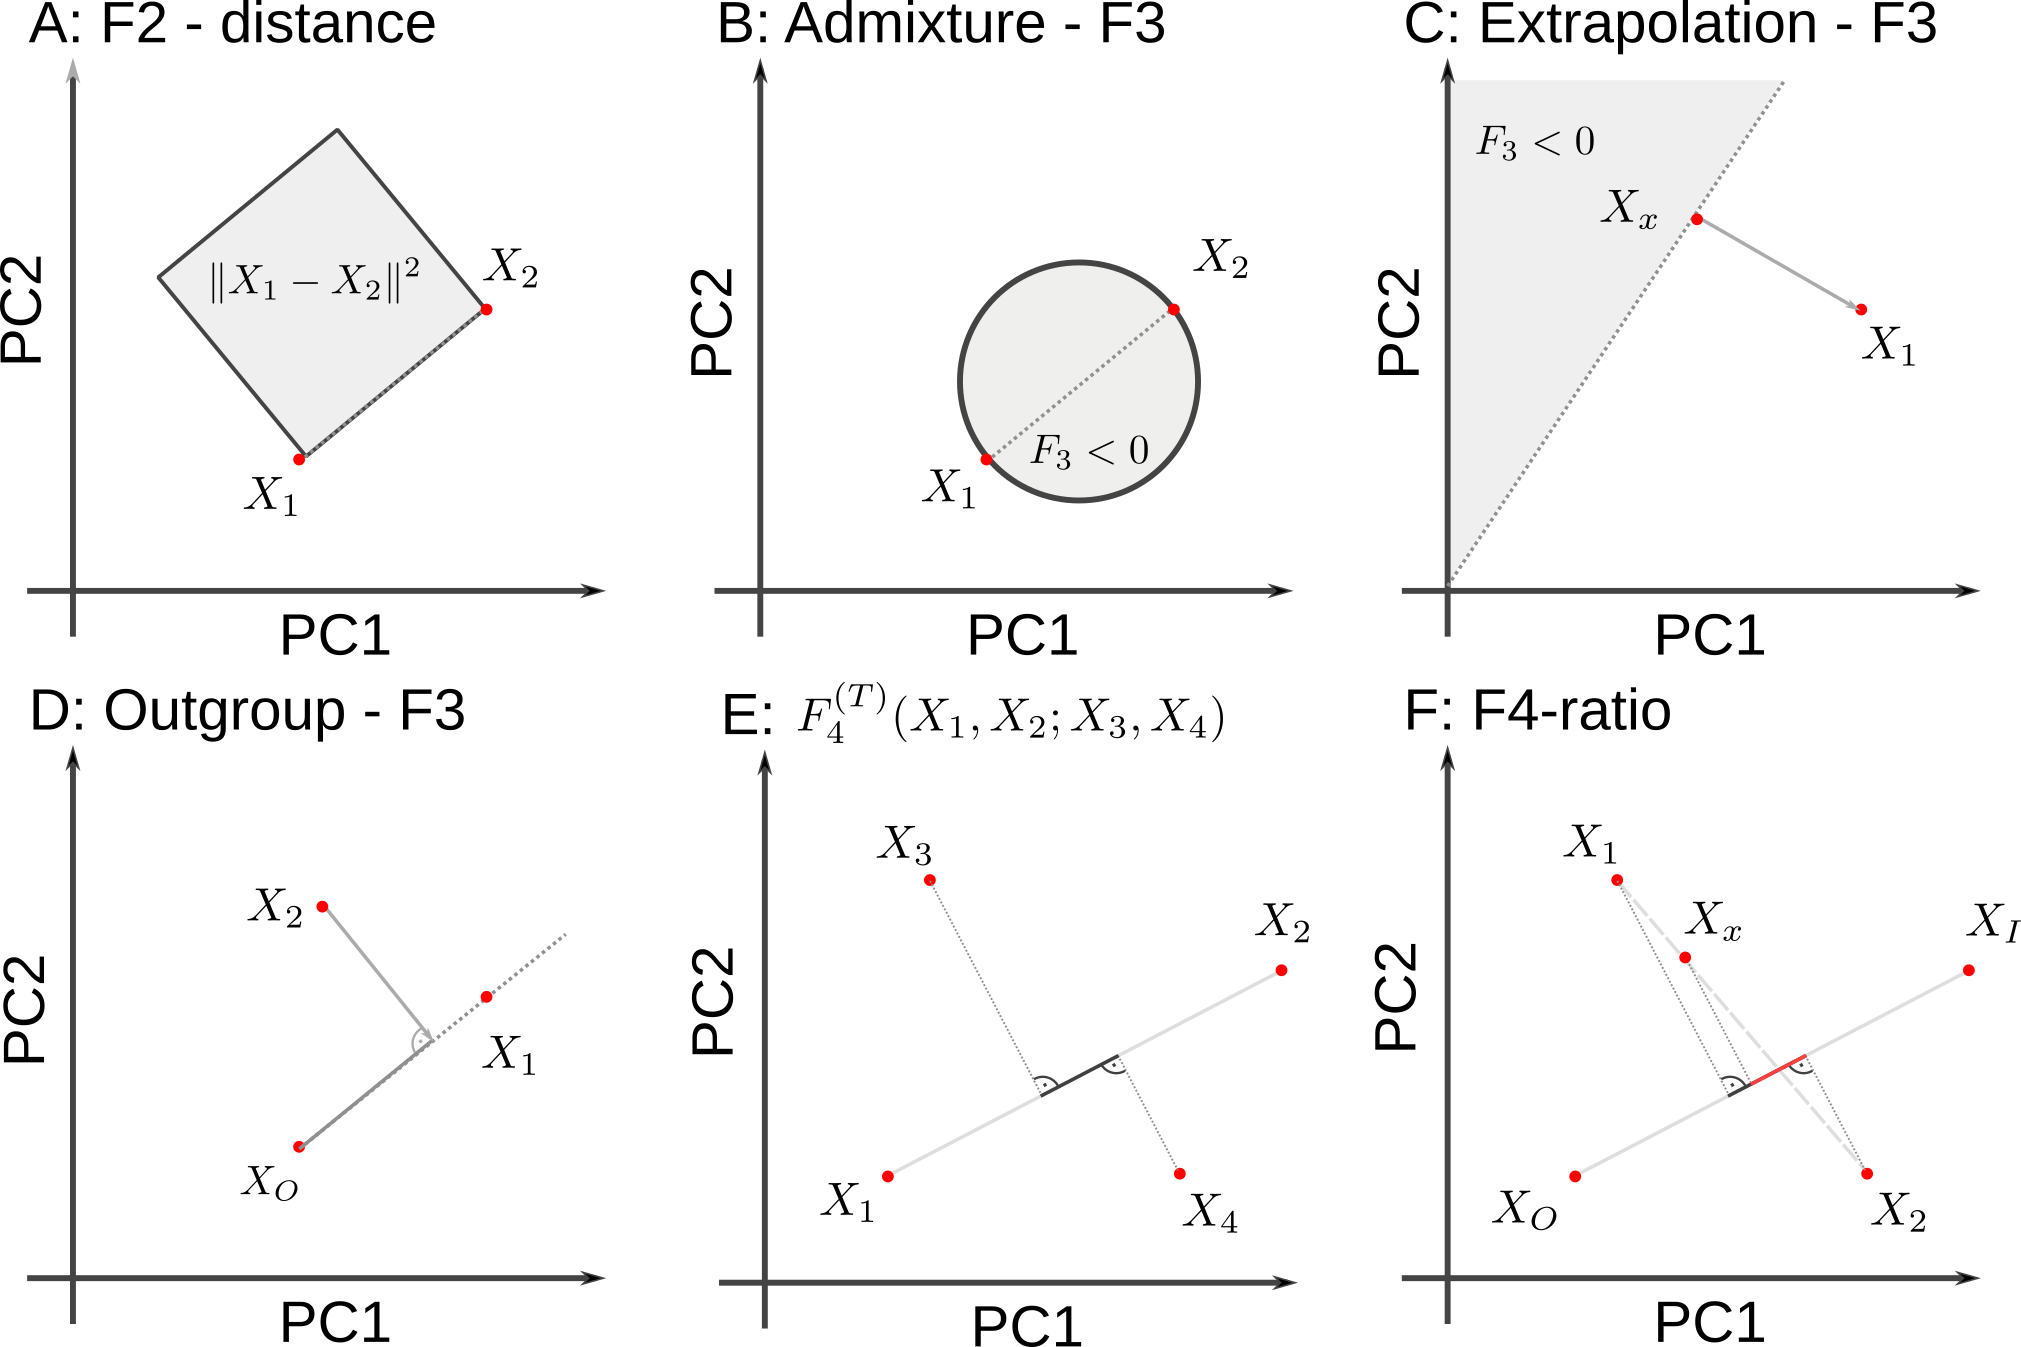
\includegraphics[width=\textwidth]{dummy_pca.png}
	\caption{\textbf{Geometric representation of $F$-statistics on 2D-PCA-plot.} A: $F_2$ represents the squared Euclidean distance between two points in PC-space. B: Admixture-$F_3(X_x; X_1, X_2)$ is negative if $X_x$ lies in the circle specified by the diameter $X_2-X_1$}. C: $F_3(X_x; X_1, X_2)$ is negative given $X_1, X_x$ if $X_2$ is in the gray space.  D: Outgroup-$F_3$ reflects the projection of $X_2 - X_O$ on $X_1 - X_O$. E: $F_4$ is the projection of $X_3 - X_4$ on $X_1-X_2$. F: If $X_x$ is admixed between $X_1$ and $X_2$, the admixture proportions will be projected.
\end{figure}

\subsubsection{$F_4$ and right angles}
The inner-product-interpretation of $F_4$ is similar to that of $F_3$, with the change that the two vectors we consider do not involve the same population. However, a finding of $F_4(X_1, X_2; X_3, X_4) = \langle X_1 - X_2, X_3 - X4 \rangle = 0$ similarly implies that the two vectors are orthogonal, and a non-zero value reflects the projection of one vector on the other.

\subsubsection{$F_4$-ratio}
\begin{eqnarray}
\frac{F_4(X_I, X_O; X_X, X_1)}{F_4(X_I, X_O; X_2, X_1)} &=& \frac{\norm{X_I-X_O}\norm{X_X-X_1}\cos(\alpha)}{\norm{X_I-X_O}\norm{X_2-X_1}\cos(\beta)}\nonumber\\
&=&\frac{\norm{X_X-X_1}\cos(\alpha)}{\norm{X_2-X_1}\cos(\beta)}\nonumber\\
&=& \frac{\norm{X_X' - X_1'}}{\norm{X_2' - X_1'}}
\end{eqnarray}
where $\alpha$ and $\beta$ are the angles between vectors, and $X_i'$ is the projection of $X_i$ on $X_I-X_O$.

Conjecture: Thus, we are measuring the distances between the admixing populations on the projected on the axis between $X_I$ and $X_O$. This ought to be valid only if $\langle X_1 - X_1', X_2 - X_2' \rangle$ are orthogonal to each other, and to $X_OX_I$, i.e.
$F_4(X_1, X_1', X_2, X_2') = 0$
 
	


	\subsection{What is a dimension?}
	In both the PCA and $F$-statistic framework, a population at  a particular point in time can be thought of as a single point in allele-frequency space, given by the $k$-dimensional vector $v_0$ of allele frequencies at the $k$ SNPs in that population. If this population evolves for some time in isolation, allele frequencies will change due to genetic drift from $v_0$ to some other point $v_1$. Likewise, a second population with frequency $w_0$ will move to $w_1$. Crucially, if these populations do not interact, the changes in allele frequency, $v_1 - v_0$ and $w_1 - w_0$ will be uncorrelated \cite{patterson2012}. Thus, if we have two populations that descend from the same ancestral population in isolation, they can be thought of as evolving along orthognal dimensions from the same point. This argument is at the foundation of F-statistics.
	
	

\section{Results}
The theory outlined in the previous section suggests that $F$-statistics have a geometric interpretation on PCA plots. In this section, I use these interpretation in the analysis of human genetic variation data set. I use two data sets based on the ``Human Origins''-SNP set (597,573 SNPs). Both are subsets of the Reich lab compendium data set v44.3, downloaded from \url{https://reich.hms.harvard.edu/allen-ancient-dna-resource-aadr-downloadable-genotypes-present-day-and-ancient-dna-data}. 

\paragraph{West-Eurasian data set}
This data set of 1,119 individuals from 62 populations contains  present-day individuals from the Eastern Mediterranean, Caucasus and Europe. It is frequently used as a basis of comparison for ancient genetic analyses of Western Eurasian individuals \cite{patterson2012}. Population genetic differentiation in this region is low and closely mirrors geography \cite{novembre2008}. 

\paragraph{World Overview data set}
This data set of 638 individuals from 33 population contains individuals throughout the world, and is used as a sparse data set capturing much of global human genetic variation. This data set spans Africa, Eurasia and the Americas, and we might therefore expect the population structure to be much more sparse.

I perform analyses at the level of populations to ease presentation, and because it is an assumption of $F$-statistics that the genetic variation with sampled population is independent of the variation between samples that I am focusing on here. I use \texttt{admixtools 2.0.0} \url{https://github.com/uqrmaie1/admixtools} to compute a matrix of $F_2$-statistics between all populations. To obtain a PC-decomposition I use equation XXX and the \texttt{eigen} function in \texttt{R}, and compare them with the $F_3$ and $F_4$-statistics calculated using admixtools 2.

\paragraph{Admixture-$F_3$}
As a first step, I plot the first two principal components of the Westeurasian data set (Figure \ref{fig:f3}A). This PCA presents two parallel clines, one from the Levant and Arabia (``BedouinB'') to the Caucasus (``Abkhasian''), and a second one from Southern (``Sardinian'') to Northeastern Europe (``Mordovian''). In this context, I examine $F_3(X; Basque, Turkish)$, i.e. a statistic that aims to ask which populations can be represented as a mixture between a Southwestern (Basque) and Southeastern (Turkish) European population. The -- largely Southern European -- populations for which the point estimate of these $F_3$-statistic is negative are highlighted in red. They both fall close to the center of the $F_3$-circle, either defined on the first two (dark grey) or all PCs (light gray). However, many populations inside the circle on the first 2 PCs, including English, Sardinians and Canary Islanders have positive $F_3$-values, on higher PCs, showing that the first two PCs do not capture all the genetic variation related to population structure for this data set. 

This is expected because for spatially continuous populations, PCA will not be sparse \cite{novembre2008a}.  Consequently, approximating $F_3$ by the first two or ten PCs (Figure \ref{fig:f3}B) only gives a coarse approximation of $F_3$, and from Figure \ref{fig:f3}C we see that many higher PCs contribute to $F_3$ statistics.

Thus, the main benefit of this PCA-plot is that it allows us to identify populations outside the circle (from the Levant and Caucasus), for which $F_3$ is guaranteed to be positive.

\paragraph{Outgroup-$F_3$}
The Outgroup-$F_3$-statistic is commonly used to infer which population is closest in a set of reference populations. In Figure \ref{fig:f3}D, I present a PCA of the world data set, with populations colored according to $F_3(Mbuti; Mozabite, X_i)$, i.e. a statistic that is commonly interpreted as finding the population $X_i$ that is most closely related to Mozabite. On a PCA, we can interpret this $F_3$ statistic as the projection of the line segment $\text{Mbuti}X_i$ onto the line through Mbuti and Mozabite (black line). For each population, the projection is indicated with a grey line. In the full data space, this line is always orthogonal to the segment Mbuti-Mozabite, but on the plot (i.e.) the subspace spanned by the first two PCs, this is only true if the relevant variation is captured by the first two PCs. We see that particularly the samples from East Asia, Siberia and the Americas project very close to orthogonally, suggesting that most of the variation is captured by these first two PCs. That the approximation of $F_3$ on 


\subsection{$F_4$}
Using $F_3$-statistics, I showed that we can think of the admixture test as a test of whether the admixed population lies in a particular $n$-ball, and the outgroup $F_3$-statistic can be thought of as a projection of the test populations on the line connecting the outgroup to the reference sample. In this section, I will develop similar interpretation of $F_4$ on PCA-plots, and to investigate sparsity. 

First, we investigate the sparsity in the world overview data set: We find that the vast amount of contribution to the statistics comes from the first two PCs (Figure \ref{fig:f4}A). For example, the correlation between $F_4(X, Y, \text{Mozabite}, \text{Yoruba})$ and its approximation using the first two PCs is 99.2\%. To visualize the interpretation of $F_4$ as an angle, we use statistics of the form $F_4(X, \text{Sardinian}; \text{Mozabite}, \text{Yoruba})$, which can be interpreted as the angle between the vectors Mozabite-Yoruba and $X$-Sardinian. In Figure \ref{fig:f4}B, I show the angle based on two (blue), ten (green) and all PCs $red$. I find that for most Asian and American populations the angle is very close to 90°, as would be expected if the variation between African and non-African populations is mostly orthogonal. On the other hand, if $X$ is an African population, the angle is lower, and much less well approximated. This demonstrates that this PCA-plot likely does not model within-African population structure adequately. 

The $F_4$-statistics for the Westeurasian data set are slightly less sparse, the correlation coefficients between $F_4(X, \text{French}; \text{Finnish}, \text{Canary Islander})$ and its approximation using the first two or three PCs is 95.5\% and 99.1\% respectively (Figure \ref{fig:f4}E). I also show that the interpretation of $F_4$ as a projection can be used as a useful visualization (Figure \ref{fig:f4}D). On the $x$-axis, I plot $\langle X; \text{Finnish}, \text{Canary Islander}\rangle$, so that the horizontal distance between all pairs of populations corresponds to their respective $F_4$-statistics $F_4(X, Y; \text{Finnish}, \text{Canary Islander})$. On the $Y$-axis and with the coloring I display the first two principal components of the residual, i.e. the genetic variation that is missed by viewing the data through this projection. We find that most European populations have positive values on residual PC1, and are relatively closely clustered. In contrast Middle Eastern and Caucasian populations have negative values on this gradient. This allows us to visualize that this particular $F_4$-projection does an adequate job if we are interested in describing European variation, but it fails to explain the non-European data. We can further quantify this by investigating the percent of variance explained on each axis (Figure \ref{fig:f4}F), where I find that the projection axis only describes around 12\% of hte variation, compared to residual PC1 with almost 30\%.


\begin{figure}[!ht]
	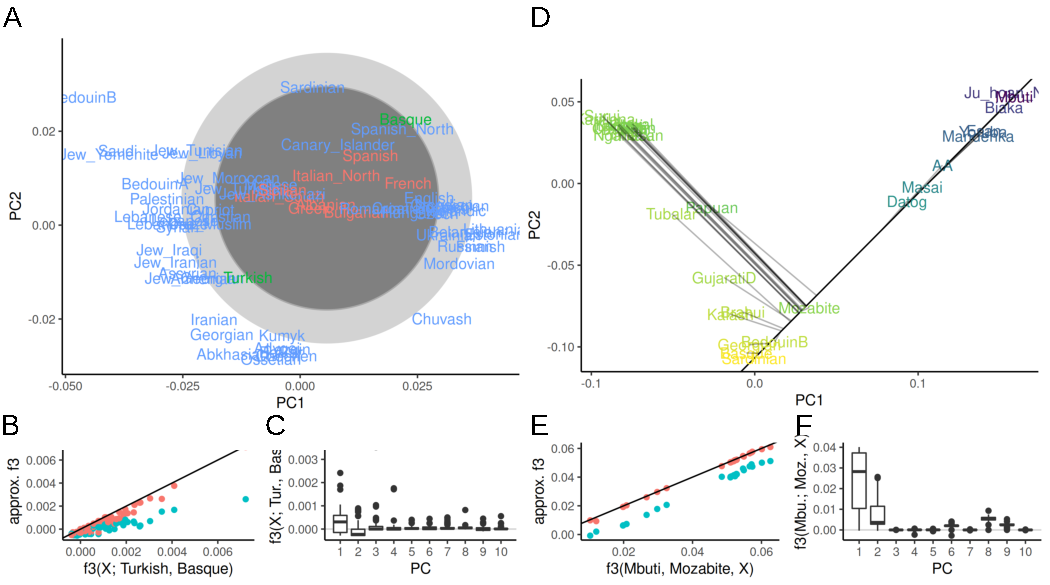
\includegraphics[width=\textwidth]{figures/fig_f3_data.pdf}
	\caption{\textbf{PCA and $F_3$-statistics} A: PCA of Western Eurasian data; the circle denotes the region for which $F_3(X; \text{Basque}, \text{Turkish})$ may be negative. Populations for which $F_3$ is negative are colored in red. B, E: $F_3$ approximated with two (blue) and ten (red) PCs versus the full spectrum. C,F: Contributions of PCs 1-10 to each $F_3$-statistic. D: PCA of World data set, color indicates value of $F_3(\text{Mbuti}; \text{Mozabite}, X)$. The black line shows the projection axis Mbuti-Mozabite, the gray lines indicates the projected position of each population. }
	\label{fig:f3}
\end{figure}

\begin{figure}[!ht]
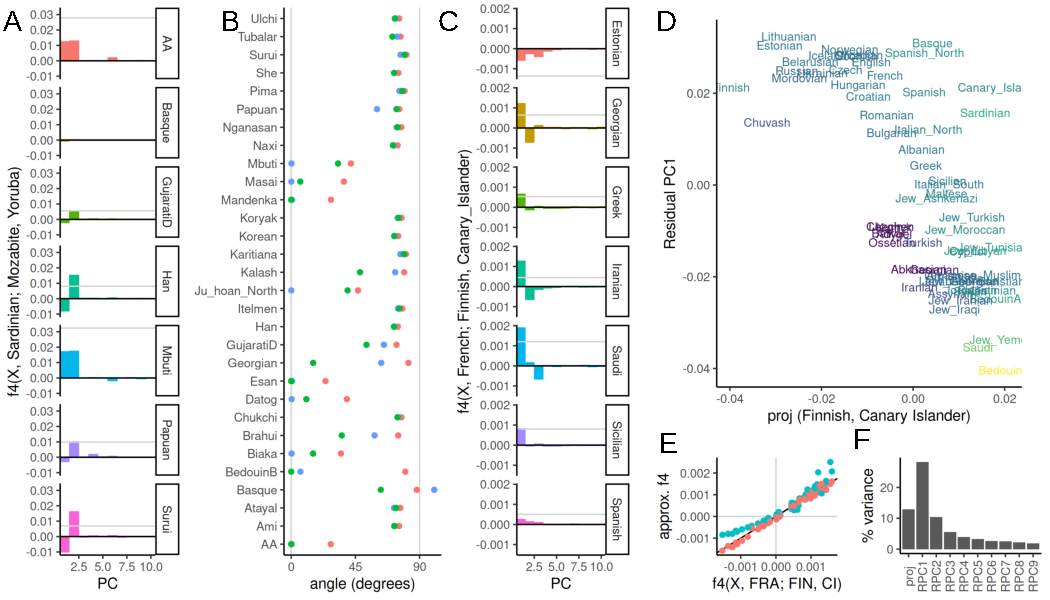
\includegraphics[width=\textwidth]{figures/fig_f4_data.pdf}	
	\caption{\textbf{PCA and $F_4$-statistics} A: Spectrum of select $F_4$-statistics in World data set. B: Projection angle representation of $F_4(X, Sardinian; Mozabite, Yoruba)$ (red) and approximations using two (blue) and ten (green) PCs. C: Spectrum of select $F-4$-statistics in Westeurasian data set. D: Scatterplot of $F_4$-projection on Finnish-Canary Islanders axis and residual PC1.
	E: $F_4(X, \text{French}, \text{Finnish}, \text{Canary Islander})$ vs. prediction using two (blue) and ten(red) PCs. F: Percent variance explained for the projection of panel D and the first nine residual PCs.
	}
\label{fig:f4}
\end{figure}

\section{Discussion}
Particularly for the analysis of ancient DNA, $F$-statistics have been established as a powerful tool to describe population genetic diversity, but they have a number of limitations. In particular, they assume that populations are discrete, related as a graph, and that gene flow between populations is rare \cite{patterson2012,harney2020}. As a consequence, researchers concerned about model fits may ascertain reference populations in a way that satisfies these assumptions, thus inadvertently making population structure appear sparser than it truly is. This is perhaps most obvious from Figure \ref{fig:f3}B, where large gaps are present. However, these gaps are due to sparse sampling that disappear if more populations were sampled \cite[e.g.][]{peter2020a}, not due to gaps in genetic diversity. If population ascertainment is not done very carefully, tools built on top of $F$-statistics, such as \texttt{qpGraph} and \texttt{qpAdm}, may thus only provide a very loose lower bound for the number of gene flow events.

In contrast, the perspective on $F$-statistics in data space \citep{oteo-garcia2021} and on PCA does not require assumptions on number of admixture or gene flow events. Independent of any model, A population $X_x$ can be thought of as admixed between $ X_1$ and $X_2$ if it lies in the ball with diameter $\overline{X_1X_2}$. And independent of any models, two axes of variation that are not perpendicular to each other shows that there is some degree of shared history. 

The connection between the graph-based and PCA-based interpretations of $F_3$ and $F_4$ is due to concept of projection. As illustrated above, both $F$-statistics can be thought of as projections on any particular axis of variation. If that variation corresponds to a tree-branch, the interpretations align. A collorary to this interpretation is the importance of orthogonality, or independence for describing gene flow. Populations without gene-flow will evolve independently, and their changes in allele frequency will therefore be orthogonal, resulting in $F_4$-statistics of zero, and right angles on a PCA plot. Even though this is only true when considering all PCs, the result holds reasonably well when just looking at the first two PCs -- in our example of the world-overview data, I found that the variation in Sub-Saharan Africa is mostly -- but not completely -- uncorrelated with the variation between European and Asian populations (Figure \ref{fig:f4}A).

While the data space produces a much larger model space than trees, the main drawback of the PCA-based interpretation is a lack of interpretability; it is not easy to define a generative model that could generate a complex PCA-plot. Thus, in the future the tree- and PCA-based interpretations will likely be used in conjunction. 

 However, despite the apparent complexity, the PC-spaces \emph{are} sparse, and using just ten or even two PCs often gives very good approximations.






To make PCA and $F$-statistics more comparable in practical settings, there are a number of -- mainly statistical -- concerns that still need to be addressed in future work. The perhaps most obvious one is that PCA is most frequently run on individuals, whereas $F$-statistics are often calculated on populations. This is not a conceptual issue, as both PCA and $F$-statistics can be run on either \cite{cavalli-sforza1994}. Population based analyses have the advantage that they are easier to interpret and compute (current packages are ill-equipped to calculate all pairwise $F$-statistics between data sets with thousands of individuals \cite{patterson2012}). However, this requires the assumption that the within-population variation is independent from the between-population variation; something that is analogous to the variance partitioning based on PCs here. 

A second difference is that frequently, rare SNPs are weighted higher in PCA, whereas all SNPs are weighted the same for $F$-statistics \cite{patterson2006}. This is only a difference of convention; $F$-statistics could also be calculated using the same weighting. The close connection between the two approaches developed here suggest that for most analyses, users might want to be consistent and use the same weighting for both types of analyses. 

The third and perhaps biggest gap are statistical issues. The treatment here focusses on the mean estimated $F$-statistic, but many  applications of $F$-statistics are based on hypothesis tests \cite{patterson2012}. This requires estimating accurate standard errors for these statistics, which is difficult since nearby SNPs will be correlated \cite{hahn2019}. In contrast, standard PCA does not modeljointly models the covariance matrix due to population structure and sampling. On the other hand, for both data sets I investigated here, the matrix $\MF$ of $F$-statistics estimated using admixtools2 is not a proper squared Euclidean distance matrix, i.e. it is not negative semidefinite and has imaginary PCs. This is not a practical when considering single $F$-statistics or PCA (for analyses here, I used a nearby matrix  \citep{higham2002} with no apparent loss of precision). It does however mean that tools that use matrices of $F$-statistics, such as \texttt{qpadm} or \texttt{qpgraph} may be ill-calibrated, which may partly explain why they generally have poor out-of-sample predictive power and are restricted to a few dozen samples at a time. A model-based framework based on probabilistic PCA \citep{meisner2021, agrawal2020, softimpute} would likely be able to generate consistent $F$-statistics and PCs, while incorporating sampling error and missing data.

\begin{itemize}
    \item weighting of SNPs
    \item estimation error
    \item propagating erros
    \item exploratory data analysis
    \item missing data
    \item population vs. sample allele frequencies
\end{itemize}

\appendix
\section{Derivation}\label{appendix:fonpc}
\begin{eqnarray}
F_2(X_i, X_j) &=& \sum_{l=1}^L \big( (x_{il} - \mu_l) -(x_{jl} -\mu_l)\big)^2 = F_2(Y_i, Y_j)\nonumber\\
&=& \sum_{l=1}^L \big( \sum_k L_{kl}P_{ik} - \sum_kL_{kl}P_{kj}\big)^2\nonumber\\
&=& \sum_{l=1}^L \left( \sum_k L_{kl} (P_{ik} -P_{jk}) \right)^2\nonumber\\
&=& \sum_{l=1}^L \left( \sum_k L_{kl}^2 (P_{ik} -P_{jk})^2 + 2\sum_{k\neq k'} L_{kl}L_{k'l}(P_{ik} - P_{jk'})^2 \right)\nonumber\\
&=& \sum_k \underbrace{\left(\sum_{l=1}^L L_{kl}^2\right)}_1 (P_{ik} -P_{jk})^2 + \sum_{k\neq k'}\underbrace{\left(\sum_{l=1}^L L_{kl}L_{k'l}\right)}_{0} (P_{ik} - P_{jk'})^2\nonumber\\
&=& \sum_k (P_{ik} - P_{jk})^2
\end{eqnarray}

In summary, the first row shows that $F_2$ on the centered data will give the same results (as distances are invariant to translations), in the second row we apply the PC-decomposition. The third row is obtained from factoring out $L_{lk}$. Row four is obtained by multiplying out the sum inside the square term for a particular $l$. We have $k$ terms when for $\binom{k}{2}$ terms for different $k$'s.  Row five is obtained by expanding the outer sum and grouping terms by $k$.The final line is obtained by recognizing that $\ML$ is an orthonormal basis; where dot products of different vectors have lengths zero.

Note that if we estimate $F_2$, unbiased estimators are obtained by subtracting the population-heterozygosities $H_i, H_j$ from the statistic. As these are scalars, they do not change above calculation.
\bibliography{main}

\end{document}
